\documentclass[a4paper]{ctexart}
\usepackage{C:/Programs/TinyTeX/mytex/yovren}
\renewcommand\covername{强\ 化\ 学\ 习}
\renewcommand\reportname{Lab2 DQN}
\renewcommand\rheadname{实\ 验\ 报\ 告}
\begin{document}
\include{C:/Programs/TinyTeX/mytex/cover_a4}
\tableofcontents
\newpage

\section{实验要求}
\begin{enumerate}
    \item 基于助教给出的代码,完善DQN算法的实现
    \item 在此基础上,实现Double DQN (DDQN), Dueling DQN, Dueling DDQN,并对DQN和它们的表现进行比较
    \begin{itemize}
        \item 绘制Reward曲线(4条:DQN, DDQN, Dueling DQN, Dueling DDQN)。为了更好的视觉效果,可以从Tensorboard中导出CSV,用seaborn等重绘
        \item 进行简要的分析,包括收敛速度、最优性、稳定性等角度
        \item 录制各方法最好策略的视频,10秒以内
    \end{itemize}
    \item 不需要太过关注训练的分数
    \item 加分项:实现Rainbow中其他改进手段,并进行对比
\end{enumerate}

\section{实验原理}

\subsection{DQN算法}
根据$Q$函数可以得到$Q(s_t,a_t)$接近$r_t+\gamma Q(s_{t+1},\pi{s_{t+1}})$,我们希望能学到这个关系,并把等式的左右边当作一个回归问题。在实现的时候,利用到两个网络,策略网络和目标网络,一开始这两个网络是一样的,在训练的时候,把目标网络固定住,只调整策略网络的参数,更新一定轮数后才把参数复制到目标网络中,目标值就变了,接下来就要重新训练。
\begin{itemize}
    \item 初始化策略网络$Q$、目标网络$\hat{Q}$,令$\hat{Q} = Q$
    \item 对于每一个回合中的每一个时间步$t$
    \begin{itemize}
        \item 对于给定状态$s_t$,用$\epsilon$-贪婪策略基于$Q$执行动作$a_t$,将($s_t,s_t,r_t,s_{t+1}$)存储到缓冲区中
        \item 从缓冲区中批量采样($s_t,s_t,r_t,s_{t+1}$)
        \item 更新$Q$的参数使得$Q(s_t,a_t)$接近$r_t+\gamma \hat{Q}(s_{t+1},max_a\hat{Q}(s_{t+1},a))$
        \item 每C次更新重置$\hat{Q} = Q$
    \end{itemize}
\end{itemize}

\subsection{DoubleDQN算法}
过估计是指估计的值函数比真实值函数要大,一般来说,Qlearning之所以存在过估计的问题,根源在于Qlearning中的最大化操作,max操作使得估计的值函数比值函数的真实值大。而且过估计量并非是均匀的,因此值函数的过估计会影响最终的策略决策,从而导致最终的策略并非最优,而只是次优。

为了解决值函数过估计问题,Hasselt提出了Double Qlearning 的方法,将动作的选择和动作的评估分别⽤不同的值函数来实现。DQN中用$\hat{Q}$评估$\hat{Q}$上最好的动作,而DoubleDQN中用$\hat{Q}$评估$Q$中最好的动作,经过这样的变换,模型在过高估计的问题上得到了缓解,稳定性也就得到了提高。

\subsection{DuelingDQN算法}
Dueling DQN则从⽹络结构上改进了 DQN。动作值函数可以分解为状态值函数和优势函数,DQN的网络直接输出Q值;而Dueling网络由公式$Q(s,a)=V(s)+A(s,a)-mean_a(A(s,a))$确定。

\subsection{Noisy Network}
我们可以在值函数中加入一定的噪声,噪声的大小影响了模型的探索特性,噪声越小表示探索能力越小,噪声越大表示探索能力越大。我们可以为$Q$和$\hat{Q}$两个模型参数分别加入噪声随机变量,与之前的$\epsilon$greedy的探索不同,Nisy Network 的探索方式更平滑,对探索的粒度控制更细腻。

\subsection{Multi-step Learning}
前面介绍的Q-Learning 大多通过下一时刻的回报和价值估计得到目标价值,这种方法在前期具有学习速度较慢的弱点,为了克服这个弱点,Multi-step Learning 使用了更多步的回报,这样在训练前期目标价值可以估计得更准确,从而加快训练速度。

\section{实验代码}
\subsection{模型:QNet和DuelingQNet}
\begin{minted}[breaklines]{python}
class QNet(nn.Module):
    def forward(self, x):
        x = self.fc1(x)
        x = F.relu(x)
        x = self.fc2(x)
        x = F.relu(x)
        x = self.fc3(x)
        return x

class DuelingQNet(nn.Module):
    def forward(self, x):
        feature = self.fc1(x)
        # 计算V(s)
        advantage = F.relu(feature)
        advantage = self.value_fc2(advantage)
        advantage = F.relu(advantage)
        advantage = self.value_fc3(advantage)
        # 计算A(s,a)
        value = F.relu(feature)
        value = self.adv_fc2(value)
        value = F.relu(value)
        value = self.adv_fc3(value)
        return value + advantage - advantage.mean()
\end{minted}

\subsection{缓冲区:ReplayBuffer}

\begin{minted}[breaklines]{python}
class ReplayBuffer:
    def sample(self, batch_size):
        # 从经验回放缓冲区中随机采样批量数据
        batch = random.sample(self.memory, batch_size)
        # 从采样的批量数据中提取状态、动作、奖励、下一个状态和完成状态
        states = torch.tensor([data.state for data in batch], dtype=torch.float).to(self.device)
        actions = torch.tensor([data.action for data in batch], dtype=torch.long).to(self.device)
        rewards = torch.tensor([data.reward for data in batch], dtype=torch.float).to(self.device)
        next_states = torch.tensor([data.next_state for data in batch], dtype=torch.float).to(self.device)
        dones = torch.tensor([data.done for data in batch], dtype=torch.uint8).to(self.device)
        return states, actions, rewards, next_states, dones
\end{minted}

\subsection{训练代理:Agent}
\begin{minted}[breaklines]{python}
class Agent:

    # 根据更新公式更新策略网络
    def learn(self, epsilon_decay):
        # 从缓冲区取样
        state_batch, action_batch, reward_batch, next_state_batch, done_batch = self.memory.sample(self.batch_size)
        # 实际Q值
        q_values = self.policy_net(state_batch).gather(dim=1, index=action_batch.unsqueeze(1)).squeeze(1)
        if not self.is_double:
            # 直接使用target网络的最大Q值
            next_q_values = self.target_net(next_state_batch).max(1)[0]
        else:
            # 使用policy网络选择动作,使用target网络计算目标Q值
            next_actions = self.policy_net(state_batch).max(1)[1].detach().unsqueeze(1)
            next_q_values = self.target_net(next_state_batch).gather(dim=1, index=next_actions).squeeze(1)
        # 预测Q值
        expected_q_values = reward_batch + self.gamma * next_q_values * (1 - done_batch)    
        pass
\end{minted}


\subsection{NoisyQNet}
\begin{minted}[breaklines]{python}
class NoisyLinear(nn.Module):
    def __init__(self, input_dim, output_dim, std_init=0.5):
        super(NoisyLinear, self).__init__()
        # 输入和输出维度
        self.input_dim = input_dim
        self.output_dim = output_dim
        # 初始标准差
        self.std_init = std_init
        # 权重的均值和标准差
        self.weight_mu = nn.Parameter(torch.FloatTensor(self.output_dim, self.input_dim))
        self.weight_sigma = nn.Parameter(torch.FloatTensor(self.output_dim, self.input_dim))
        self.register_buffer('weight_epsilon', torch.FloatTensor(self.output_dim, self.input_dim))
        # 偏置的均值和标准差
        self.bias_mu = nn.Parameter(torch.FloatTensor(self.output_dim))
        self.bias_sigma = nn.Parameter(torch.FloatTensor(self.output_dim))
        self.register_buffer('bias_epsilon', torch.FloatTensor(self.output_dim))
        # 初始化参数和噪声
        self.reset_parameter()
        self.reset_noise()

    def reset_parameter(self):
        # 初始化参数
        nn.init.kaiming_uniform_(self.weight_mu, a=math.sqrt(5))
        fan_in, _ = nn.init._calculate_fan_in_and_fan_out(self.weight_mu)
        bound = 1 / math.sqrt(fan_in)
        nn.init.uniform_(self.bias_mu, -bound, bound)
        nn.init.constant_(self.weight_sigma, self.std_init / math.sqrt(self.input_dim))
        nn.init.constant_(self.bias_sigma, self.std_init / math.sqrt(self.input_dim))

    def reset_noise(self):
        # 重置噪声的权重
        epsilon_in = torch.randn(self.input_dim)
        epsilon_out = torch.randn(self.output_dim)
        self.weight_epsilon.copy_(epsilon_out.ger(epsilon_in))
        # 重置噪声的偏置
        self.bias_epsilon.copy_(torch.randn(self.output_dim))

    def forward(self, input):
        if self.training:
            # 训练模式下,添加噪声
            weight = self.weight_mu + self.weight_sigma.mul(self.weight_epsilon)
            bias = self.bias_mu + self.bias_sigma.mul(self.bias_epsilon)
        else:
            # 推理模式下,使用均值参数
            weight = self.weight_mu
            bias = self.bias_mu
        return F.linear(input, weight, bias)
\end{minted}

\subsection{NStepRelayBuffer}
\begin{minted}[breaklines]{python}
class ReplayBuffer:
    def __init__(self, capacity, n_step, gamma, device):
        self.capacity = capacity
        self.n_step = n_step
        self.gamma = gamma
        # 经验回放缓冲区
        self.memory = deque(maxlen=self.capacity)
        # 存储N步经验的缓冲区
        self.n_step_buffer = deque(maxlen=self.n_step)
        self.device = device

    def _get_n_step_info(self):
        # 从N步经验缓冲区获取N步信息的方法
        reward, next_state, done = self.n_step_buffer[-1][-3:]  # 获取最后一个元素的奖励、下一个状态和完成状态
        for _, _, rew, next_s, do in reversed(list(self.n_step_buffer)[:-1]):
            # 从后向前计算N步经验的奖励、下一个状态和完成状态
            reward = self.gamma * reward * (1 - do) + rew
            reward, next_state, done = (rew, next_s, do) if do else (reward, next_state, done)
        return reward, next_state, done

    def store(self, state, action, reward, next_state, done):
        # 存储经验到经验回放缓冲区
        self.n_step_buffer.append((state, action, reward, next_state, done))  # 将经验添加到N步经验缓冲区
        if len(self.n_step_buffer) < self.n_step:
            return  # 如果N步经验缓冲区未填满,则返回

        # 获取N步信息
        reward, next_state, done = self._get_n_step_info()
        state, action = self.n_step_buffer[0][:2]  # 获取第一个元素的状态和动作
        # 将N步经验存储到经验回放缓冲区
        self.memory.append((state, action, reward, next_state, done))
\end{minted}


\section{实验结果}
\subsection{Double和Dueling的效果}
\begin{figure}[H]
    \centering
    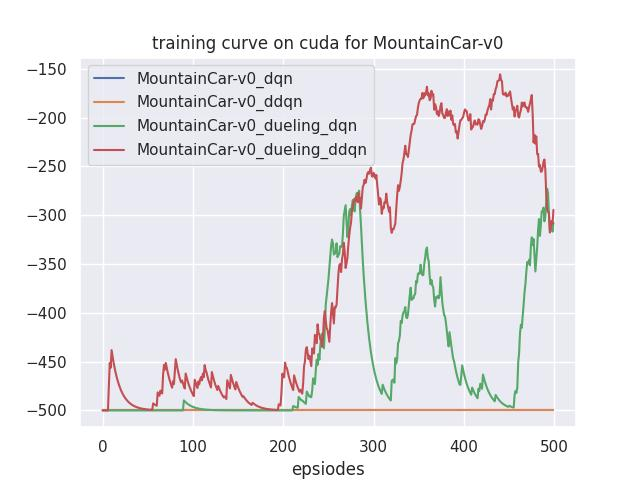
\includegraphics[width=0.46\textwidth]{train.jpg}
    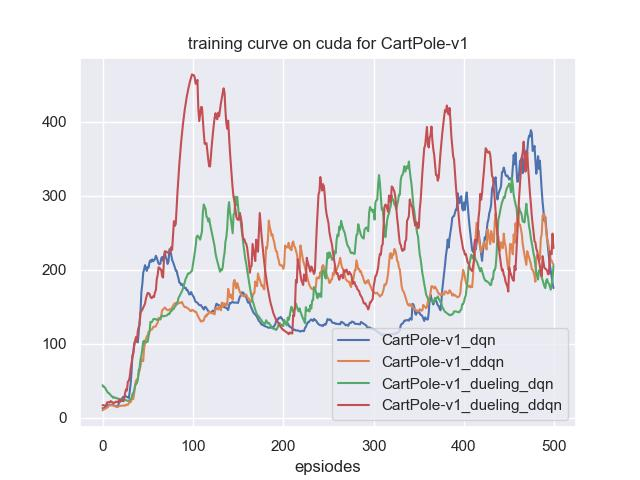
\includegraphics[width=0.46\textwidth]{train2.jpg}
    \caption{第一次实验}
    \label{a}
\end{figure}
\begin{figure}[H]
    \centering
    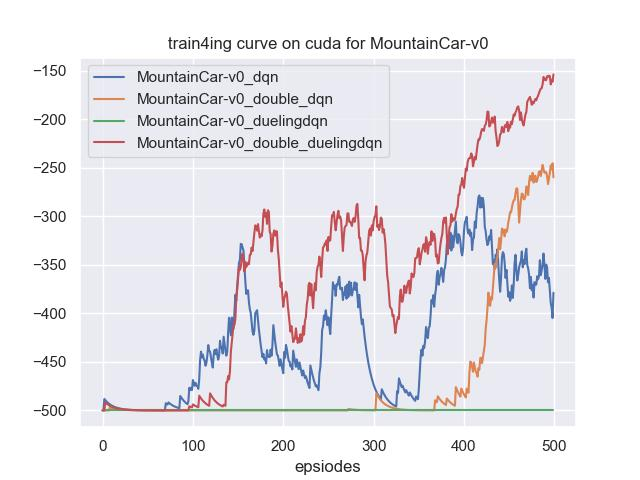
\includegraphics[width=0.46\textwidth]{train8.jpg}
    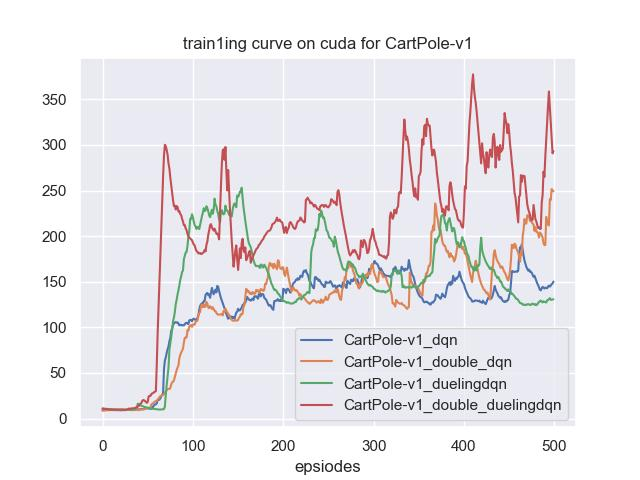
\includegraphics[width=0.46\textwidth]{train5.jpg}
    \caption{第二次实验}
    \label{b}
\end{figure}
如图\ref{a}和图\ref{b}所示分别是在两个任务上分别做了两次相同实验后的reward变化趋势,可以明显看到dueling\_doubledqn的表现最好,收敛速度最快,曲线总体呈上升趋势且比较稳定,其次表现较好的是double\_dqn,说明double操作确实一定程度上减少了过估计,且duelingdqn也比dqn表现更好。但是总的来说,这四次实现的reward都不能稳定上升,特别是在Cartpole-v1任务上结果波动较大,推测出现这一结果一方面由于是模型对于CatPole任务来说太过简单,导致容易过拟合,另一方面可能和epsilon和learning\_rate等超参数的设置有关,因此设置了另一组对比试验来验证这些超参数对实验的影响。

\subsection{超参数的影响}
实验首先在CartPole任务上针对是否使用epsilon\_decay策略和learning\_rate的选择设置了对比试验,结果如下
\begin{figure}[H]
    \centering
    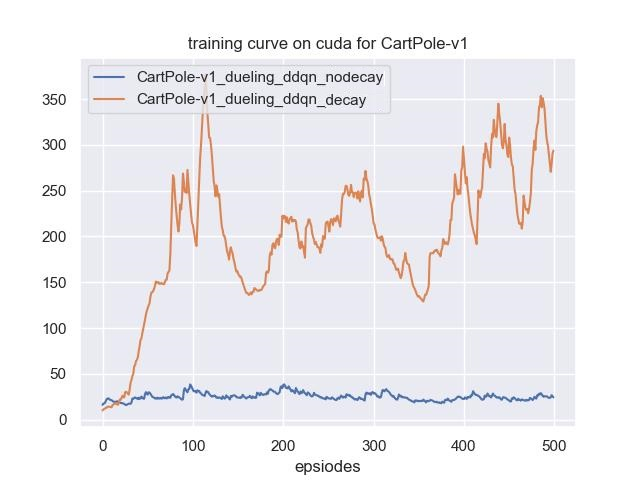
\includegraphics[width=0.46\textwidth]{train3.jpg}
    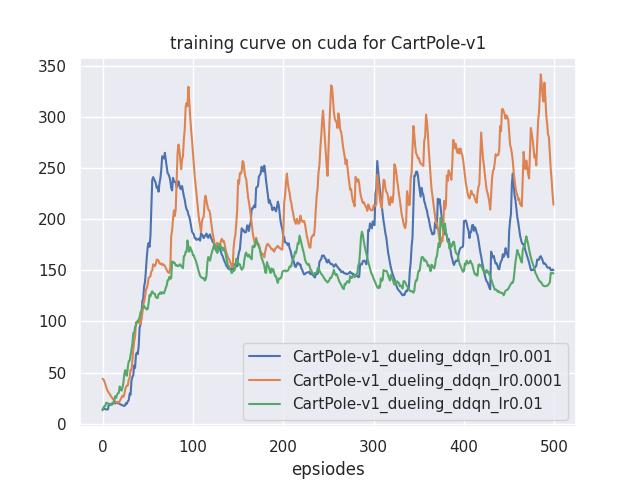
\includegraphics[width=0.46\textwidth]{train4.jpg}
    \caption{超参数对比试验}
    \label{c}
\end{figure}
如图\ref{c}所示是两组实验上的reward变化趋势,可以明显看到对于CartPole任务来说选择epsilon\_decay的表现更好,固定学习率选择0.0001表现更优。为了我探究在不同任务上是否都有这样的结论,我们在CartPole和MountainCar两个任务上针对是否使用epsilon\_decay策略,是否使用learning\_rate\_scheduler策略继续设置了对比试验。

如图\ref{d}所示,对于不同任务甚至不同的模型来说,可能需要不同的策略组合,对于MountainCar来说使用epsilon\_decay策略或learning\_rate\_scheduler策略都会使效果降低,但是对于CartPole来说,learning\_rate\_scheduler策略对结果的帮助很明显,epsilon\_decay策略对结果影响不大,这需要针对不同的任务设置和模型进行特定分析选择。

\subsection{改进方法的影响}
\begin{figure}[H]
    \centering
    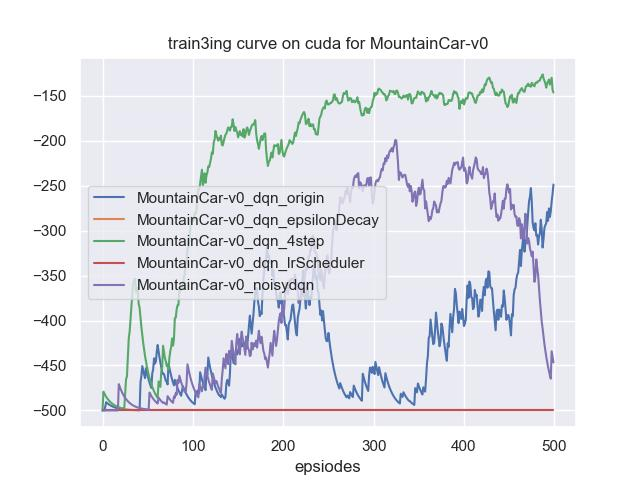
\includegraphics[width=0.46\textwidth]{train6.jpg}
    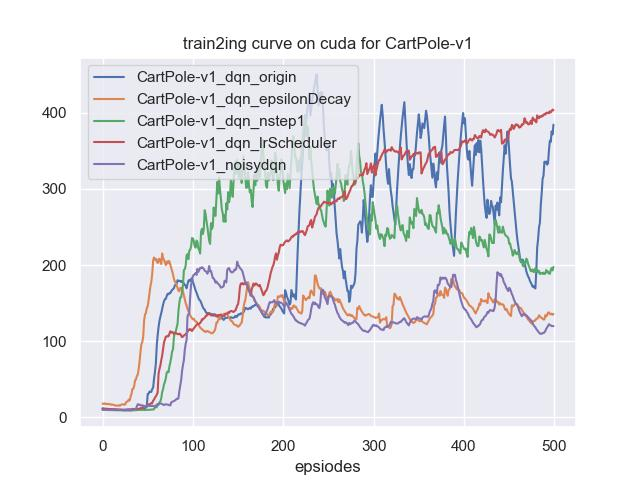
\includegraphics[width=0.46\textwidth]{train7.jpg}
    \caption{超参数和改进方法对比试验}
    \label{d}
\end{figure}
如图\ref{d}所示是不同改进方法对实验的影响,可以明显看到对于MountainCar任务来说,使用4step\ learn对结果的帮助很大,无论是收敛速度还是稳定性都有很大的提升,noisydqn也能使收敛速度变快,而对于CartPole任务来说,相比于基准设置,添加4step\_learn能使reward上升更稳定,收敛速度加快,但是noisydqn的整体reward不如原始dqn。


\section{实验总结}
本次实验实现了实验要求的基本部分,并且实现了加分点multi-step和noisydqn,除此之外,为了探究不同超参数设置对实验的影响,在实验要求以外针对超参数进行了对比试验寻找最优配置,最终对实验结果进行了曲线展示和视频录制等多方式的展示和分析对比,最终实验取得了不错的效果,同时也加深了对DQN的理解。

\end{document}